Podemos establecer una relación entre las coordenadas rectangulares y las polares mediante la construcción de un punto ${\left(x,y\right)}$ en un plano bidimensional, como se muestra en la siguiente ilustración:

\begin{figure}[H]
  \centering
  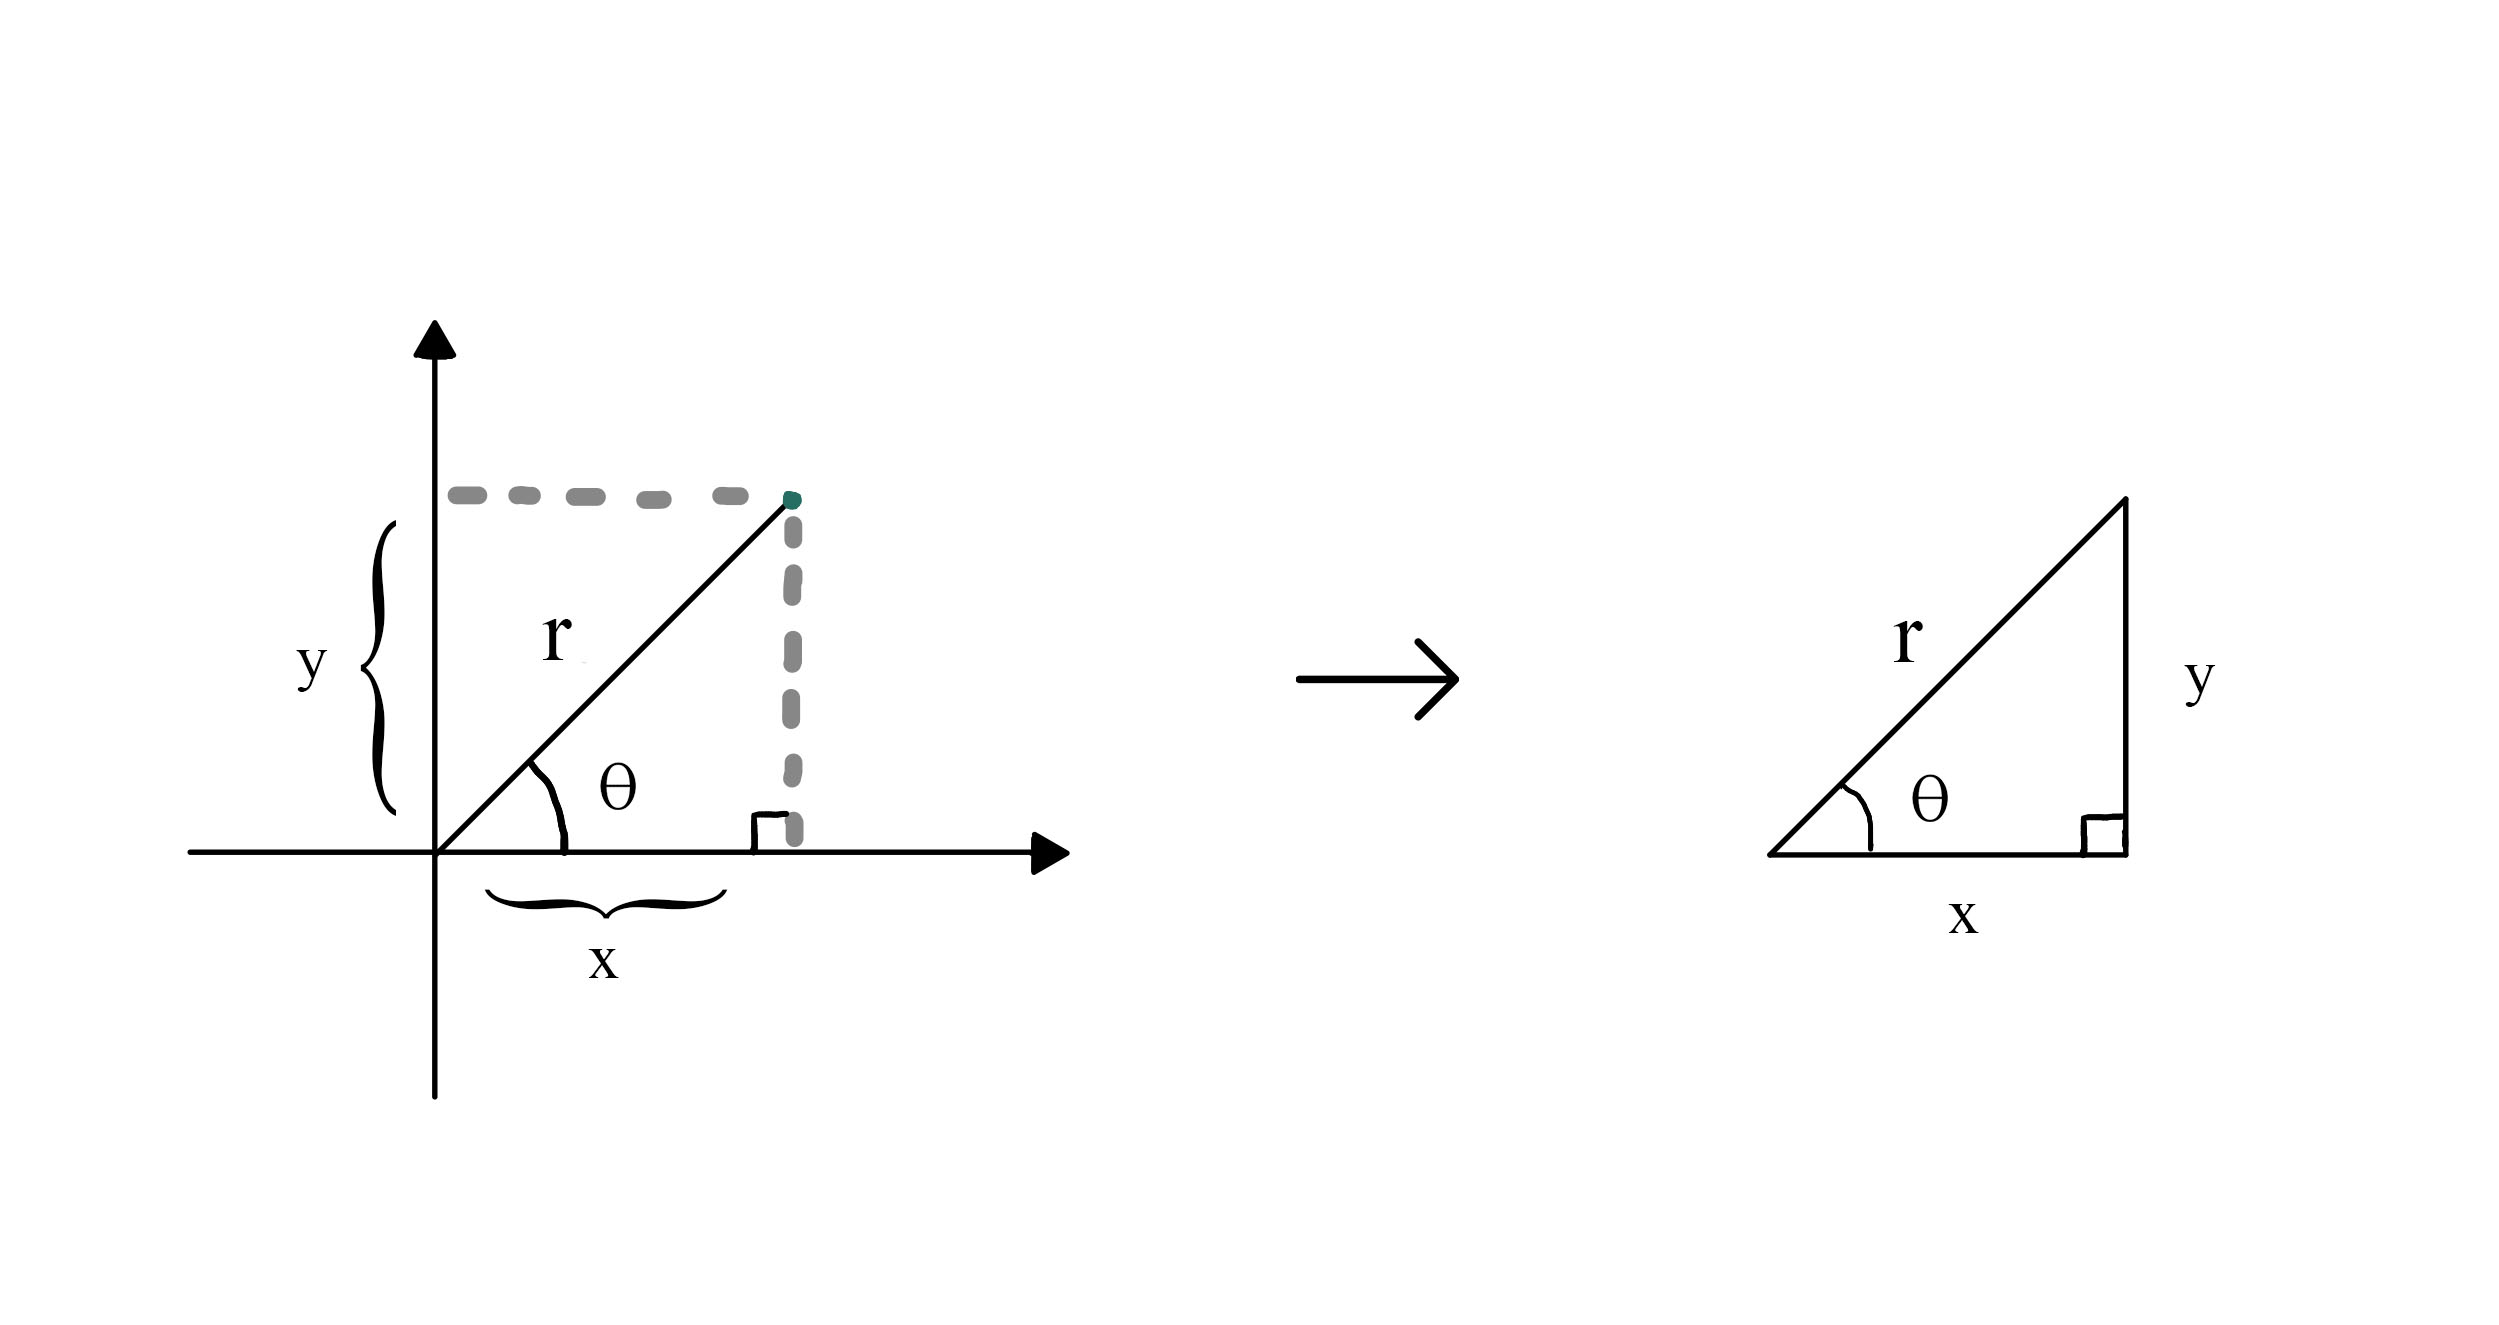
\includegraphics[width=11.17cm, height=5.67cm]{img/graph/relacion_r}
  \caption{Relación de coordenadas rectangulares y polares.}
  \label{relacion_de_coordenadas}
\end{figure}

Donde ${r}$ representa la distancia desde el origen hasta el punto y el ángulo es ${\theta}$. Por tanto, existe la coordenada polar ${\left(r,\theta\right)}$, donde el origen permanece igual y el eje polar se representa como el mismo eje x. De ésta manera, se forma un triángulo rectángulo y se tienen las siguientes relaciones:

\begin{eqnarray*}
  \cos\theta = \frac{\text{cateto adyacente}}{\text{hipotenusa}} = \frac{x}{r} &\rightarrow x = r\cos\theta\\\\
  \sin\theta = \frac{\text{cateto opuesto}}{\text{hipotenusa}} = \frac{y}{r} &\rightarrow y = r\sin\theta\\\\
  \tan\theta = \frac{\text{cateto opuesto}}{\text{cateto adyacente}} = \frac{y}{x} &\rightarrow \theta = \tan^{-1}\left(\frac{y}{x}\right)
\end{eqnarray*}

\vspace{4mm}
Dichas relaciones serán útiles cuando se intente establecer los métodos de transformación de coordenadas.
